\begin{frame}{Motivazioni}
\begin{columns}
\begin{column}{0.5\textwidth}

\includegraphics[height=0.5\textheight]{motivazioni/intro_1.png}
\end{column}
\begin{column}{0.5\textwidth}
\only<1>{
\begin{quote}
    how can we build tiny little robots that are able to enter the human body through natural orifices or small incisions, to reach places minimally invasively for surgery?
    \begin{flushright}
    \tiny{---Jessica Burgner-Kahrs}
    \end{flushright}
\end{quote}
}
\only<2>{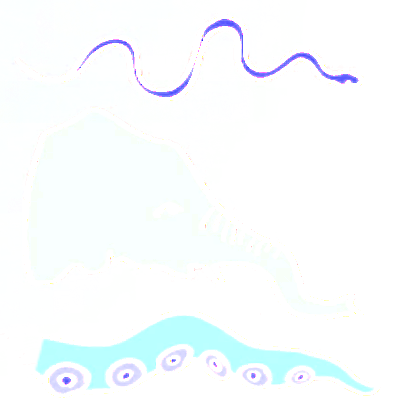
\includegraphics[height=0.5\textheight]{motivazioni/intro_2.png}}
\end{column}
\end{columns}
\Reference{Task-specific Design of Tubular Continuum Robots for Surgical Applications}{Burgner-Kahrs}{2015}

\note{
Manipolatori che entrano nel corpo per operare in modo minimamente invasivo. \\

Robot continui, ispirati alle forme presenti in natura.\\

Struttura capace di piegarsi in ogni punto. \\
}

\end{frame}

